\section{Introduction}
\noindent\rule[\linienAbstand]{\linewidth}{\linienDickeDick}

\subsection{What is Statistical Quality and Process Control}
\noindent\rule[\linienAbstand]{\linewidth}{\linienDicke}
\textbf{Definition of Quality}\\
\begin{itemize}
  \item Quality means fitness for use. and
  \item Quality is inversely proportional to variability.
  \item My definition: Something is of quality if \emph{Is} and \emph{should} are the same.
\end{itemize}

\textbf{Statistical Process Control (SPC)}\\
Statistical process control is commonly understood as a way to optimise production and manufacturing processes.\\

\textbf{The Magnificent Seven}\\
The magnificent seven are the following seven statistical (graphical) methods for analysing data:
\begin{enumerate}
  \item histogram
  \item check sheet
  \item Pareto chart
  \item defect concentration diagram
  \item cause-and-effect diagram
  \item control chart
  \item scatter diagram
\end{enumerate}

\textbf{Check Sheet}\\
The check sheet is a simple method of quality control. As a rule, it consists of a ready-made form to register and count possible problems in a production process.\\
\begin{table}[H]
  \scriptsize
  \centering
  \begin{tabular}{l|cccc|l}
    causes            & \multicolumn{4}{l|}{interruptions/quarter} &  \\
                      & 1. & 2. & 3. & 4. & total \\ \hline
    drop phone        & 1  & 0  & 0 & 2  & 3\\
    battery empty     & 3  & 3  & 2 & 4  & 12\\
    driving in tunnel & 12 & 10 & 13 & 9 & 44\\
    press button      & 1  & 1  & 0  & 3 & 5\\
    accident          & 1  & 0  & 0  & 0 & 1\\
    phone broken      & 1  & 0  & 2  & 1 & 4\\
    no obvious reason & 3  & 4  & 3  & 5 & 15
  \end{tabular}
\end{table}

\textbf{Pareto Chart}\\
The Pareto chart is a special histogram, which is used to apply the causes of a problem in function from the greatest to the least serious. It is a statistical tool for visualizing the 80-20 principle.
\begin{figure}[H]
  \centering
  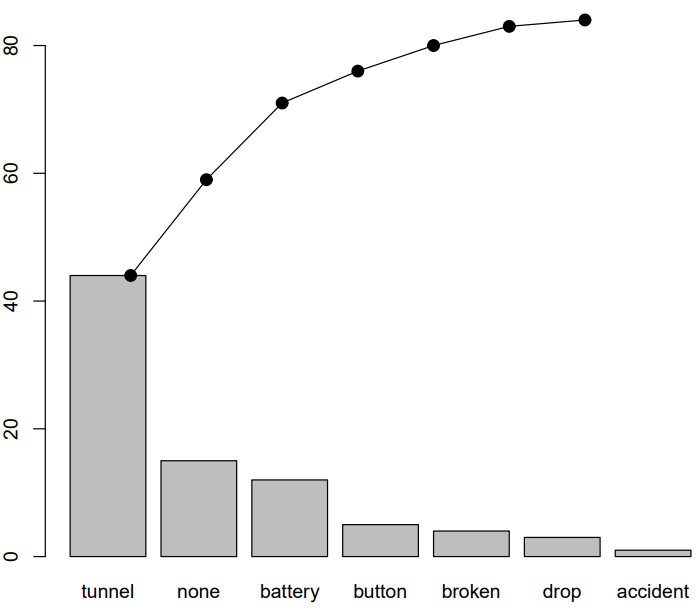
\includegraphics[width = 0.4\linewidth]{Pics/1.2.2.png}
  \caption{Pareto chart.}
\end{figure}

\textbf{Defect Concentration Diagram, Location Plot}\\
The graphical counterpart to the check sheet is the defect concentration diagram or the location plot. The diagram is used to graphically visualise the locations of the various defects on a physical object.
\begin{figure}[H]
  \centering
  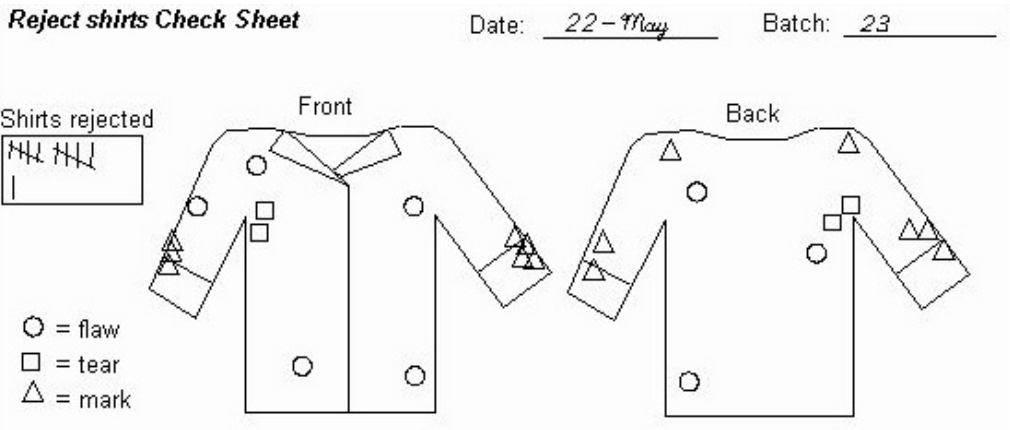
\includegraphics[width = 0.6\linewidth]{Pics/1.2.3.png}
  \caption{Defect concentration diagram or location plot: The locations of the various defects in the quality control of shirts are marked.}
\end{figure}

\textbf{Cause-and-Effect Diagram}\\
The cause-and-effect diagram is a tool in the form of a fishbone for the systematic identification of causes which make problems.
\begin{figure}[H]
  \centering
  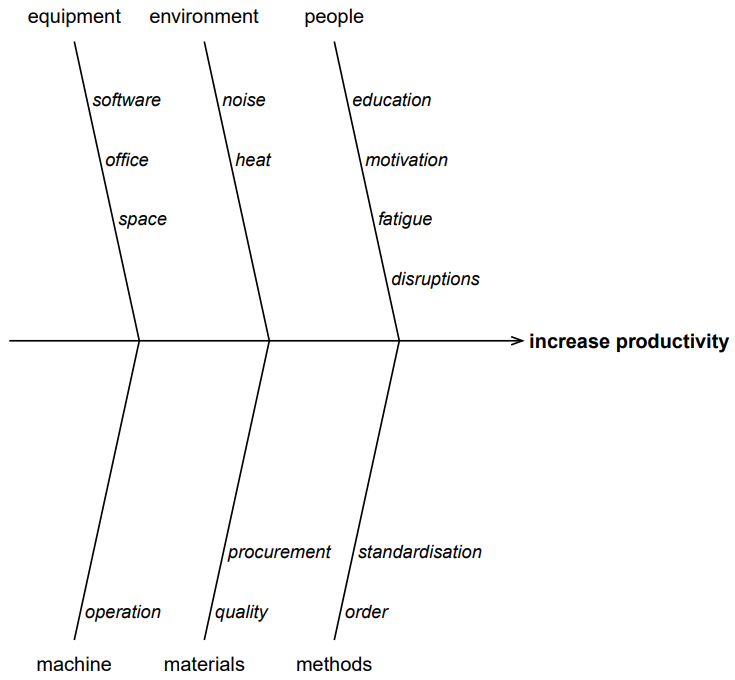
\includegraphics[width = 0.4\linewidth]{Pics/1.2.4.png}
  \caption{Cause-and-effect diagram.}
\end{figure}
